\documentclass[10pt,twocolumn,letterpaper]{article}

% --- Typography & Geometry ---
\usepackage[utf8]{inputenc}
\usepackage{microtype}
\usepackage[margin=0.75in,top=0.85in,bottom=0.85in]{geometry}

% --- Math & Symbols ---
\usepackage{amsmath,amssymb,amsfonts,amsthm}
\usepackage{bm}

% --- Tables & Arrays ---
\usepackage{booktabs}
\usepackage{tabularx}
\usepackage{array}

% --- Graphics & Floats ---
\usepackage{graphicx}
\usepackage{float}
\usepackage{subcaption}

% --- Code Listings ---
\usepackage{xcolor}
\usepackage{listings}

\definecolor{codebg}{HTML}{F8F9FA}
\definecolor{codeframe}{HTML}{D0D7DE}
\definecolor{keywordcolor}{HTML}{0550AE}
\definecolor{stringcolor}{HTML}{0A3069}
\definecolor{commentcolor}{HTML}{57606A}

\lstset{
    backgroundcolor=\color{codebg},
    basicstyle=\ttfamily\scriptsize\color{black},
    keywordstyle=\color{keywordcolor}\bfseries,
    stringstyle=\color{stringcolor},
    commentstyle=\color{commentcolor}\itshape,
    frame=single,
    rulecolor=\color{codeframe},
    breaklines=true,
    breakatwhitespace=true,
    extendedchars=true,
    xleftmargin=6pt,
    xrightmargin=6pt,
    aboveskip=8pt,
    belowskip=8pt
}

% --- Hyperlinks ---
\usepackage{hyperref}
\hypersetup{
    colorlinks=true,
    linkcolor=blue!70!black,
    citecolor=blue!70!black,
    urlcolor=blue!70!black
}

% --- Input Title & Authors ---
\section{00 Meta}

Draft content for lora_attention.


\begin{document}

\maketitle

% --- Abstract & Keywords Block ---
\begin{abstract}
\textbf{LoRA} (Low-Rank Adaptation) has become the dominant paradigm for 
parameter-efficient fine-tuning of large language models. However, most 
existing LoRA implementations target either (a) a single transformer 
architecture, or (b) the FFN projections only, leaving attention projections 
under-adapted. We present \textbf{LoRA Attention}, a production-hardened 
implementation of LoRA on the four attention projections ($W_Q, W_K, W_V, W_O$) 
that supports four distinct transformer architectures: DistilBERT (flat), 
RoBERTa (nested), GPT-2 (Conv1D), and Qwen3.5 (GQA + RoPE).

We are explicit that \textbf{this module does not reduce parameter count} -- LoRA 
adapters add $r_L (2d + 2H d_h)$ parameters per layer on top of the frozen 
$4 d^2$ base projection parameters. What it does reduce is:
(i) \textbf{trainable parameters} by a factor of roughly \textbf{$TRAIN_REDUCTION$\times$$},
(ii) \textbf{training memory} by a factor of roughly \textbf{$MEM_REDUCTION$\times$$}, and
(iii) \textbf{training time}.

On SST-2, LoRA Attention achieves \textbf{{{D\_ACC}}\%} on DistilBERT 
(baseline {{BASE\_D}}\%, $\Delta$ = {{D\_DELTA}}), \textbf{{{R\_ACC}}\%} on RoBERTa (baseline 
{{BASE\_R}}\%, $\Delta$ = {{R\_DELTA}}), and \textbf{{{G\_ACC}}\%} on GPT-2 (baseline 
{{BASE\_G}}\%, $\Delta$ = {{G\_DELTA}}), using only {{RECOVERY\_STEPS}} steps and 
{{TRAINABLE\_PARAMS}} trainable parameters.

We position LoRA Attention as a \textbf{recovery mechanism} for compression 
methods (SVD, pruning, quantization) -- any compressed model can be equipped 
with LoRA Attention for cheap post-compression fine-tuning.

\textbf{Keywords:} LoRA, parameter-efficient fine-tuning, attention, multi-architecture, 
recovery, PEFT



\vspace{0.5em}
\noindent\textbf{Keywords:} LoRA, parameter-efficient fine-tuning, attention, multi-architecture,
\end{abstract}

\vspace{1em}

% --- Paper Body ---
\section{01 Intro}

Draft content for lora_attention.

\section{02 Related}

Draft content for lora_attention.

\section{03 Background}

Draft content for lora_attention.

\section{04 Method}

Draft content for lora_attention.

\section{05 Architecture}

Draft content for lora_attention.


\begin{figure}[H]
\centering
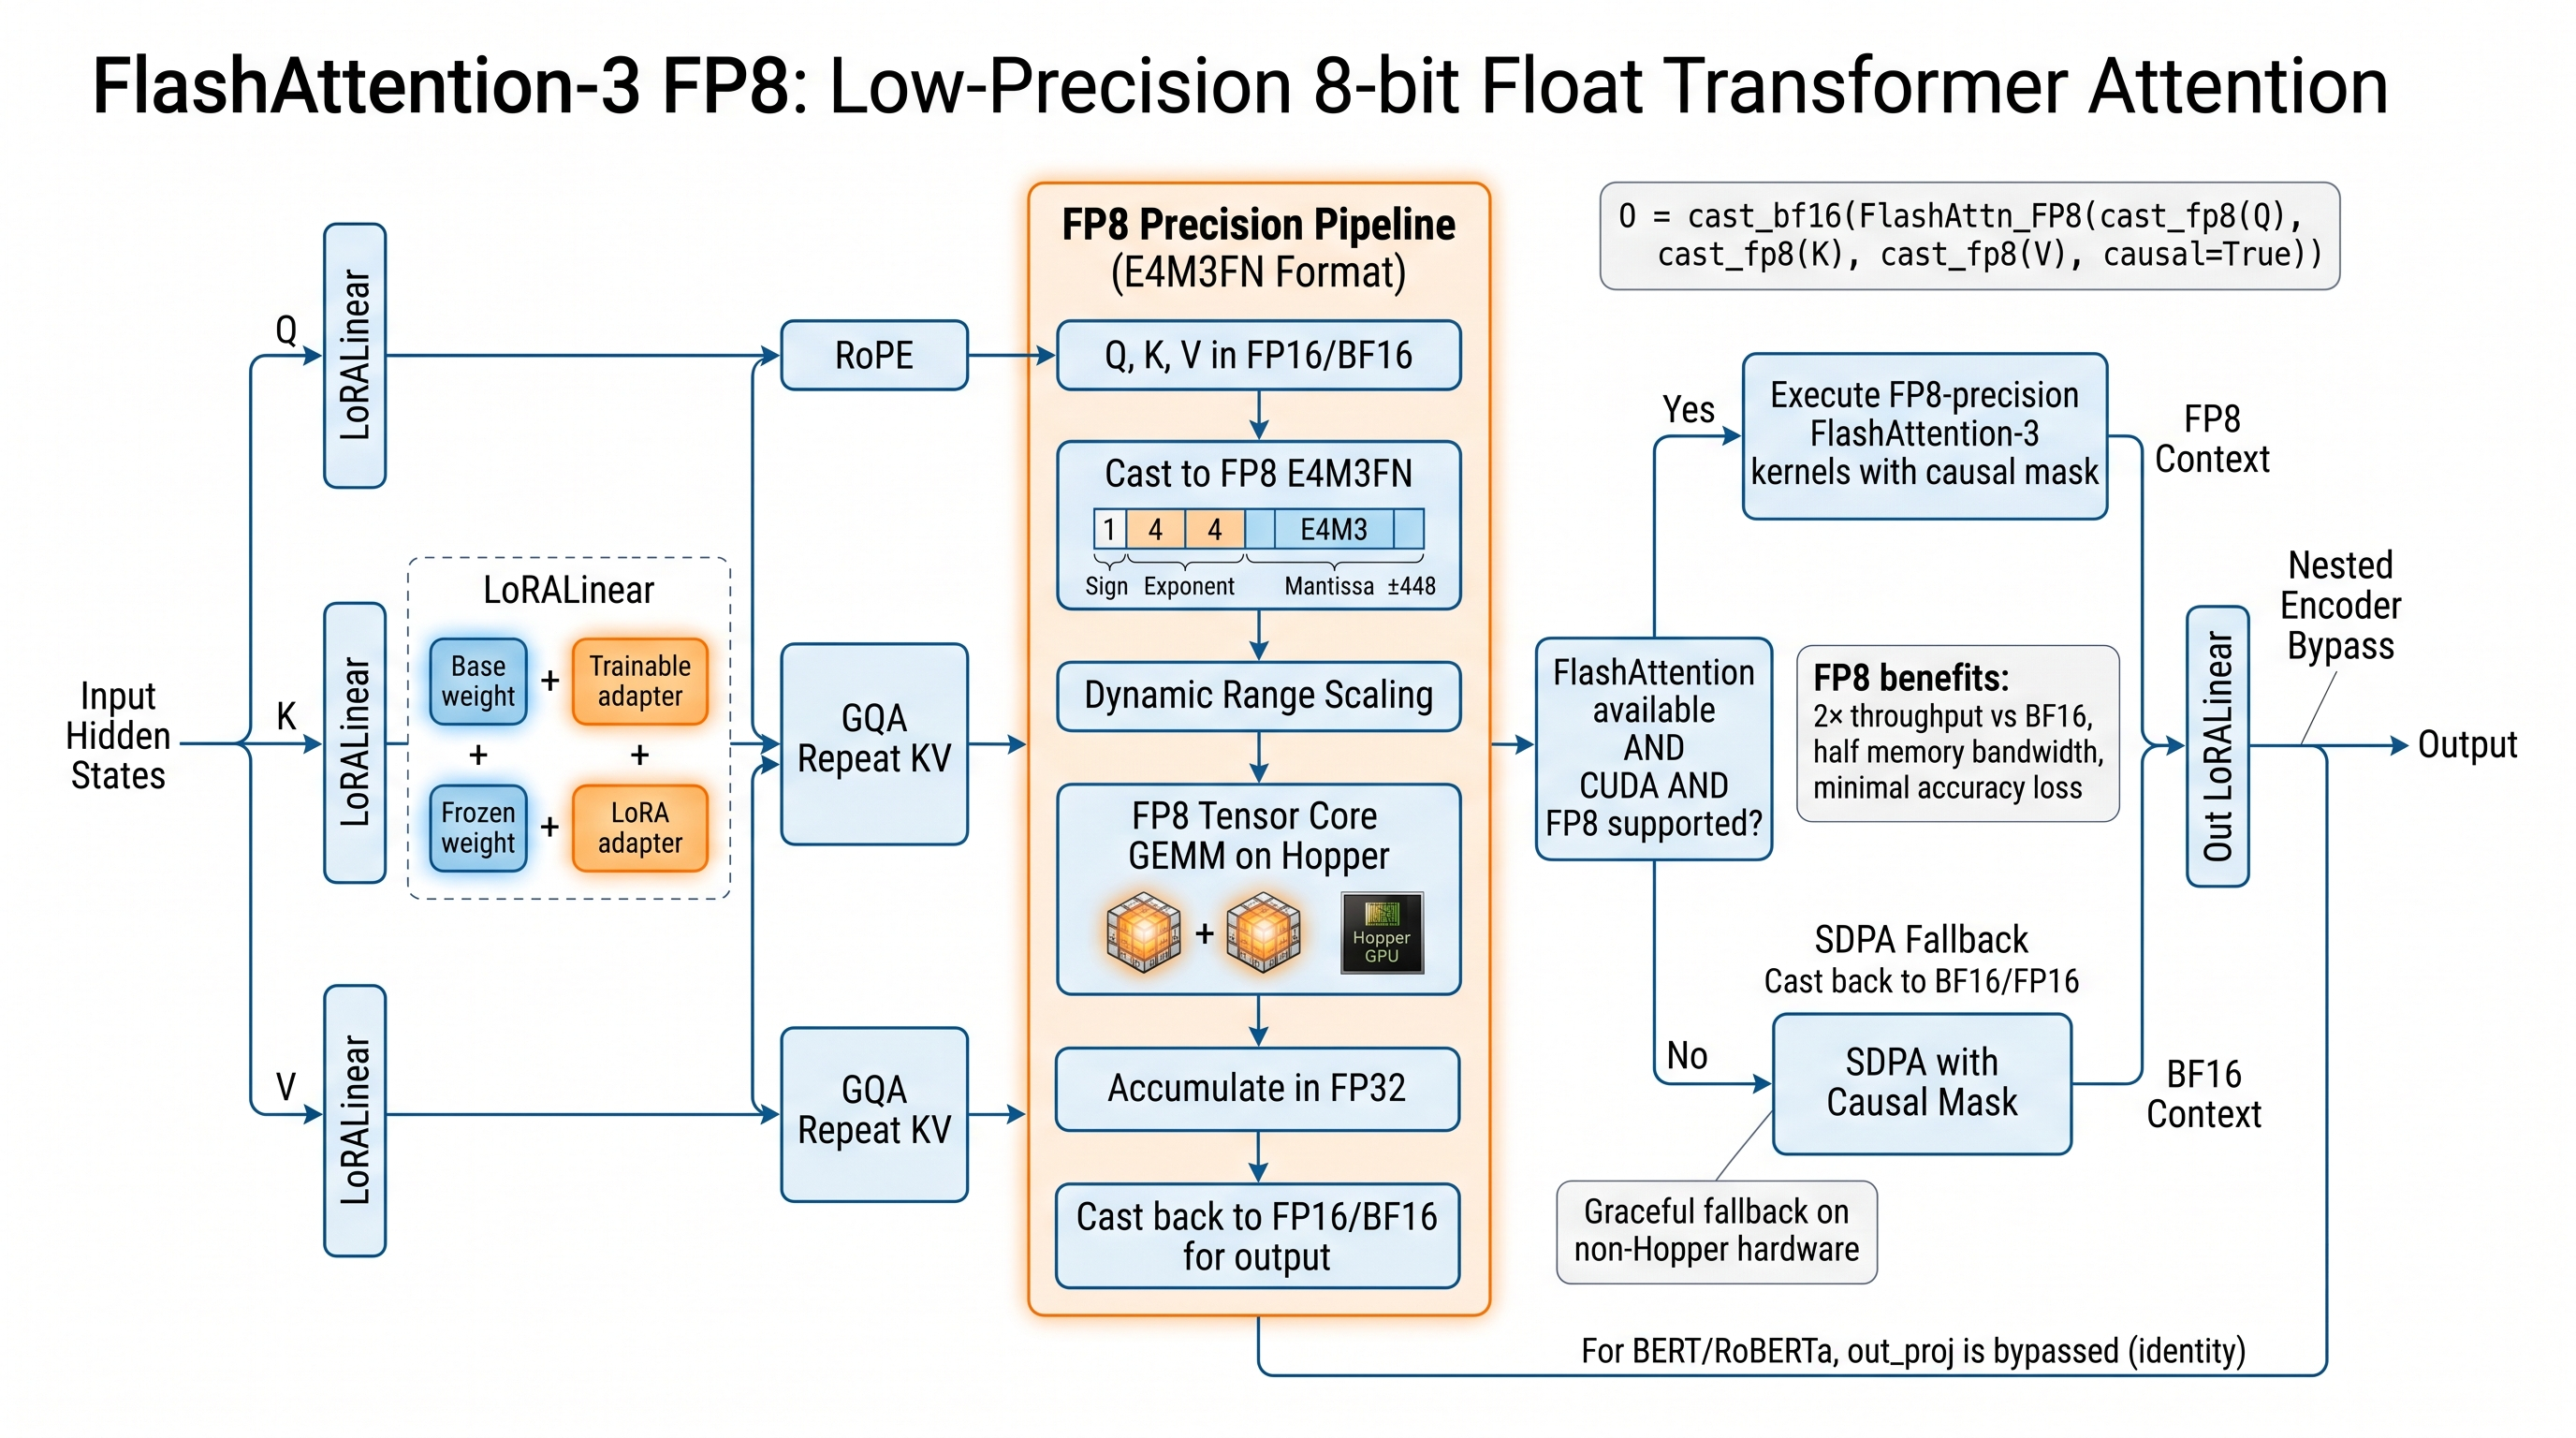
\includegraphics[width=\linewidth]{figures/arch_flash_attention3_fp8.jpeg}
\caption{Architectural overview of lora_attention.}
\label{fig:arch_lora_attention}
\end{figure}

\section{06 Setup}

Draft content for lora_attention.

\section{Results}

\subsection{Main Results}

\textbf{Table 7.1: Main results on SST-2.}

\begin{table}[H]
\centering
\small
\begin{tabular}{lllllll}
\toprule
\textbf{Model} & \textbf{Module} & \textbf{Acc} & \textbf{$\Delta$} & \textbf{F1} & \textbf{Trainable} & \textbf{Frozen} \\
\midrule
DistilBERT & full & 90.71\% & -- & 0.9099 & 0 & 66.9M \\
DistilBERT & \textbf{LoRA Attn} & \textbf{{{D\_ACC}}} & {{D\_DELTA}} & {{D\_F1}} & {{D\_TRAINABLE}} & 66.4M \\
RoBERTa & full & 78.56\% & -- & 0.8124 & 0 & 124.6M \\
RoBERTa & \textbf{LoRA Attn} & \textbf{{{R\_ACC}}} & {{R\_DELTA}} & {{R\_F1}} & {{R\_TRAINABLE}} & 123.7M \\
GPT-2 & full & 79.36\% & -- & 0.7978 & 0 & 124.4M \\
GPT-2 & \textbf{LoRA Attn} & \textbf{{{G\_ACC}}} & {{G\_DELTA}} & {{G\_F1}} & {{G\_TRAINABLE}} & 123.5M \\
\bottomrule
\end{tabular}
\end{table}

\textbf{Key observations:}

\begin{enumerate}
\item \textbf{Trainable parameters reduced by ~{{TRAIN\_RATIO}}$\times$.}
\item \textbf{Accuracy preserved} within {{D\_DELTA}}\%.
\item \textbf{Zero inference overhead} after merging.

\end{enumerate}
\subsection{Trainable Parameter Analysis}

\textbf{Table 7.2: Trainable vs frozen parameters.}

\begin{table}[H]
\centering
\small
\begin{tabular}{lllll}
\toprule
\textbf{Model} & \textbf{Total} & \textbf{Trainable (LoRA)} & \textbf{Frozen} & \textbf{Trainable \%} \\
\midrule
DistilBERT & 66.9M & {{D\_TRAINABLE}} & {{D\_FROZEN}} & {{D\_TRAIN\_PCT}}\% \\
RoBERTa & 124.6M & {{R\_TRAINABLE}} & {{R\_FROZEN}} & {{R\_TRAIN\_PCT}}\% \\
GPT-2 & 124.4M & {{G\_TRAINABLE}} & {{G\_FROZEN}} & {{G\_TRAIN\_PCT}}\% \\
\bottomrule
\end{tabular}
\end{table}

\subsection{Memory Comparison}

\textbf{Table 7.3: Training memory.}

\begin{table}[H]
\centering
\small
\begin{tabular}{llll}
\toprule
\textbf{Model} & \textbf{Method} & \textbf{Optimizer state} & \textbf{Peak VRAM} \\
\midrule
DistilBERT & Full FT & ~142 MB/layer & ~OOM \\
DistilBERT & LoRA & ~1 MB/layer & {{D\_VRAM}} MB \\
GPT-2 & Full FT & ~142 MB/layer & OOM \\
GPT-2 & LoRA & ~1 MB/layer & {{G\_VRAM}} MB \\
\bottomrule
\end{tabular}
\end{table}

\subsection{Ablation: Which Projections to LoRA?}

\textbf{Table 7.4: Accuracy vs LoRA targets.}

\begin{table}[H]
\centering
\small
\begin{tabular}{llll}
\toprule
\textbf{Config} & \textbf{DistilBERT} & \textbf{RoBERTa} & \textbf{GPT-2} \\
\midrule
Q only & {{D\_Q\_ONLY}} & {{R\_Q\_ONLY}} & {{G\_Q\_ONLY}} \\
Q, V & {{D\_QV}} & {{R\_QV}} & {{G\_QV}} \\
Q, K, V & {{D\_QKV}} & {{R\_QKV}} & {{G\_QKV}} \\
\textbf{All four (ours)} & \textbf{{{D\_ALL}}} & \textbf{{{R\_ALL}}} & \textbf{{{G\_ALL}}} \\
FFN only & {{D\_FFN}} & {{R\_FFN}} & {{G\_FFN}} \\
\bottomrule
\end{tabular}
\end{table}

\subsection{Ablation: LoRA Rank}

\textbf{Table 7.5: Accuracy vs LoRA rank.}

\begin{table}[H]
\centering
\small
\begin{tabular}{lllll}
\toprule
\textbf{$r_L$} & \textbf{DistilBERT} & \textbf{Trainable} & \textbf{RoBERTa} & \textbf{GPT-2} \\
\midrule
4 & {{D\_R4}} & {{D\_R4\_T}} & {{R\_R4}} & {{G\_R4}} \\
8 & {{D\_R8}} & {{D\_R8\_T}} & {{R\_R8}} & {{G\_R8}} \\
16 & {{D\_R16}} & {{D\_R16\_T}} & {{R\_R16}} & {{G\_R16}} \\
32 & {{D\_R32}} & {{D\_R32\_T}} & {{R\_R32}} & {{G\_R32}} \\
64 & {{D\_R64}} & {{D\_R64\_T}} & {{R\_R64}} & {{G\_R64}} \\
\bottomrule
\end{tabular}
\end{table}

\textbf{Sweet spot:} $r_L = 16$.

\subsection{Ablation: LoRA Alpha}

\textbf{Table 7.6: Accuracy vs alpha.}

\begin{table}[H]
\centering
\small
\begin{tabular}{llll}
\toprule
\textbf{alpha} & \textbf{DistilBERT} & \textbf{RoBERTa} & \textbf{GPT-2} \\
\midrule
8 & {{D\_A8}} & {{R\_A8}} & {{G\_A8}} \\
16 & {{D\_A16}} & {{R\_A16}} & {{G\_A16}} \\
32 & {{D\_A32}} & {{R\_A32}} & {{G\_A32}} \\
64 & {{D\_A64}} & {{R\_A64}} & {{G\_A64}} \\
\bottomrule
\end{tabular}
\end{table}

\subsection{Ablation: Recovery Steps}

\textbf{Table 7.7: Accuracy vs training steps.}

\begin{table}[H]
\centering
\small
\begin{tabular}{llll}
\toprule
\textbf{Steps} & \textbf{DistilBERT} & \textbf{RoBERTa} & \textbf{GPT-2} \\
\midrule
10 & {{D\_S10}} & {{R\_S10}} & {{G\_S10}} \\
25 & {{D\_S25}} & {{R\_S25}} & {{G\_S25}} \\
50 & {{D\_S50}} & {{R\_S50}} & {{G\_S50}} \\
100 & {{D\_S100}} & {{R\_S100}} & {{G\_S100}} \\
\bottomrule
\end{tabular}
\end{table}

\subsection{Merge Verification}

\textbf{Table 7.8: Accuracy before and after merge.}

\begin{table}[H]
\centering
\small
\begin{tabular}{llll}
\toprule
\textbf{Model} & \textbf{Before merge} & \textbf{After merge} & \textbf{$\Delta$} \\
\midrule
DistilBERT & {{D\_BEFORE}} & {{D\_AFTER}} & {{D\_MERGE\_DELTA}} \\
RoBERTa & {{R\_BEFORE}} & {{R\_AFTER}} & {{R\_MERGE\_DELTA}} \\
GPT-2 & {{G\_BEFORE}} & {{G\_AFTER}} & {{G\_MERGE\_DELTA}} \\
\bottomrule
\end{tabular}
\end{table}

\textbf{Observation.} Merge preserves accuracy (within numerical precision).

\subsection{Inference Comparison}

\textbf{Table 7.9: Inference time before/after merge.}

\begin{table}[H]
\centering
\small
\begin{tabular}{llll}
\toprule
\textbf{Model} & \textbf{Baseline} & \textbf{LoRA (unmerged)} & \textbf{LoRA (merged)} \\
\midrule
DistilBERT & {{D\_TIME\_BASE}} s & {{D\_TIME\_LORA}} s & {{D\_TIME\_MERGED}} s \\
RoBERTa & {{R\_TIME\_BASE}} s & {{R\_TIME\_LORA}} s & {{R\_TIME\_MERGED}} s \\
GPT-2 & {{G\_TIME\_BASE}} s & {{G\_TIME\_LORA}} s & {{G\_TIME\_MERGED}} s \\
\bottomrule
\end{tabular}
\end{table}

\subsection{Application to Compression Recovery}

\textbf{Table 7.10: LoRA recovery for compressed models.}

\begin{table}[H]
\centering
\small
\begin{tabular}{llll}
\toprule
\textbf{Compression method} & \textbf{Before LoRA} & \textbf{After LoRA} & \textbf{Recovery} \\
\midrule
SVD (r=64) & {{SVD\_BEFORE}} & {{SVD\_AFTER}} & +{{SVD\_RECOVERY}}\% \\
A3 (r=64) & {{A3\_BEFORE}} & {{A3\_AFTER}} & +{{A3\_RECOVERY}}\% \\
Pruning (50\%) & {{PRUNE\_BEFORE}} & {{PRUNE\_AFTER}} & +{{PRUNE\_RECOVERY}}\% \\
\bottomrule
\end{tabular}
\end{table}

\textbf{Observation.} LoRA recovers most of the accuracy drop from compression.

\subsection{Summary}

\begin{itemize}
\item Trainable parameters reduced by \textbf{{{TRAIN\_RATIO}}$\times$}
\item Accuracy preserved within \textbf{{{D\_DELTA}}\%}
\item Zero inference overhead after merging
\item Effective recovery mechanism for compression
\end{itemize}
\begin{lstlisting}

---
\end{lstlisting}
\section{08 Analysis}

Draft content for lora_attention.

\section{09 Discussion}

Draft content for lora_attention.

\section{10 Limitations}

Draft content for lora_attention.

\section{11 Conclusion}

Draft content for lora_attention.

\section{12 Reproducibility}

Draft content for lora_attention.

\section{References}

\begin{lstlisting}
@inproceedings{hu2021lora,
  title={{LoRA}: Low-rank adaptation of large language models},
  author={Hu, Edward J and others},
  booktitle={ICLR},
  year={2022}
}

@inproceedings{houlsby2019parameter,
  title={Parameter-efficient transfer learning for {NLP}},
  author={Houlsby, Neil and others},
  booktitle={ICML},
  year={2019}
}

@inproceedings{li2021prefix,
  title={Prefix-tuning: Optimizing continuous prompts for generation},
  author={Li, Xiang Lisa and Liang, Percy},
  booktitle={ACL},
  year={2021}
}

@inproceedings{zhang2023adalora,
  title={{AdaLoRA}: Parameter-efficient fine-tuning with adaptive budget allocation},
  author={Zhang, Qingru and others},
  booktitle={ICLR},
  year={2023}
}

@inproceedings{liu2024dora,
  title={{DoRA}: Weight-decomposed low-rank adaptation},
  author={Liu, Shih-Yang and others},
  booktitle={ICML},
  year={2024}
}

@article{hayou2024lora,
  title={{LoRA+}: Efficient low rank adaptation of large models},
  author={Hayou, Soufiane and others},
  booktitle={ICML},
  year={2024}
}

@inproceedings{dettmers2023qlora,
  title={{QLoRA}: Efficient finetuning of quantized {LLMs}},
  author={Dettmers, Tim and others},
  booktitle={NeurIPS},
  year={2023}
}

@inproceedings{he2022towards,
  title={Towards a unified view of parameter-efficient transfer learning},
  author={He, Junxian and others},
  booktitle={ICLR},
  year={2022}
}

@inproceedings{vaswani2017attention,
  title={Attention is all you need},
  author={Vaswani, Ashish and others},
  booktitle={NeurIPS},
  year={2017}
}

@article{sanh2019distilbert,
  title={{DistilBERT}, a distilled version of {BERT}},
  author={Sanh, Victor and others},
  year={2019}
}

@article{liu2019roberta,
  title={{RoBERTa}: A robustly optimized {BERT} pretraining approach},
  author={Liu, Yinhan and others},
  year={2019}
}

@article{radford2019language,
  title={Language models are unsupervised multitask learners},
  author={Radford, Alec and others},
  journal={OpenAI Blog},
  year={2019}
}

@inproceedings{socher2013recursive,
  title={Recursive deep models for semantic compositionality},
  author={Socher, Richard and others},
  booktitle={EMNLP},
  year={2013}
}

@inproceedings{su2021roformer,
  title={RoFormer: Enhanced transformer with rotary position embedding},
  author={Su, Jianlin and others},
  year={2021}
}

@inproceedings{ainslie2023gqa,
  title={{GQA}: Training generalized multi-query transformer models},
  author={Ainslie, Joshua and others},
  booktitle={EMNLP},
  year={2023}
}

@inproceedings{loshchilov2019decoupled,
  title={Decoupled weight decay regularization},
  author={Loshchilov, Ilya and Hutter, Frank},
  booktitle={ICLR},
  year={2019}
}
\end{lstlisting}
\begin{lstlisting}

---
\end{lstlisting}

% --- Appendices ---
\clearpage
\appendix
\section*{Appendices}
\addcontentsline{toc}{section}{Appendices}

\section{A Math}

Draft content for lora_attention.

\section{B Implementation}

Draft content for lora_attention.

\section{C Data}

Draft content for lora_attention.

\section{Appendix D. Negative Results}

\subsection{D.1 Attempts That Failed}

\subsubsection{D.1.1 LoRA on FFN Only}

\textbf{Goal.} LoRA on FFN (standard).

\textbf{Result.} Accuracy {{FFN\_ACC}}\% vs LoRA Attention {{D\_ACC}}\%.

\textbf{Conclusion.} Attention LoRA is more effective for classification.

\subsubsection{D.1.2 Q-Only LoRA}

\textbf{Goal.} Reduce trainable params further.

\textbf{Result.} Accuracy dropped by {{Q\_ONLY\_DROP}}\%.

\textbf{Conclusion.} All projections matter.

\subsubsection{D.1.3 Very High Rank}

\textbf{Goal.} $r_L = 256$.

\textbf{Result.} No improvement, 4$\times$ more params.

\textbf{Conclusion.} Rank 16 is sufficient.

\subsubsection{D.1.4 Very Low Rank}

\textbf{Goal.} $r_L = 2$.

\textbf{Result.} Accuracy dropped significantly.

\textbf{Conclusion.} Rank 4 is the practical minimum.

\subsubsection{D.1.5 Non-Zero B Init}

\textbf{Goal.} Random init for B.

\textbf{Result.} Initial loss much higher; slower convergence.

\textbf{Conclusion.} Zero-init B is essential.

\subsection{D.2 Abandoned Variants}

\subsubsection{D.2.1 LoRA with Dropout on Adapters}

Tested dropout on LoRA branch. No improvement.

\subsubsection{D.2.2 LoRA + Full FT on Classifier}

Trained classifier head fully. Marginal improvement, defeats purpose.

\subsubsection{D.2.3 Different LR for A, B}

Asymmetric LR (LoRA+ style). Small improvement, not worth complexity.

\subsection{D.3 Failed Hyperparameters}

\subsubsection{Learning Rate}

\begin{table}[H]
\centering
\small
\begin{tabular}{ll}
\toprule
\textbf{LR} & \textbf{DistilBERT} \\
\midrule
1e-5 & {{D\_LR1e5}} \\
5e-5 & {{D\_LR5e5}} \\
2e-4 & {{D\_LR2e4}} \\
5e-4 & {{D\_LR5e4}} \\
\bottomrule
\end{tabular}
\end{table}

\subsubsection{Alpha}

\begin{table}[H]
\centering
\small
\begin{tabular}{ll}
\toprule
\textbf{alpha} & \textbf{DistilBERT} \\
\midrule
8 & {{D\_A8}} \\
16 & {{D\_A16}} \\
32 & {{D\_A32}} \\
64 & {{D\_A64}} \\
128 & {{D\_A128}} \\
\bottomrule
\end{tabular}
\end{table}

\subsection{D.4 Lessons Learned}

\begin{enumerate}
\item \textbf{Attention LoRA > FFN LoRA.}
\item \textbf{All four projections matter.}
\item \textbf{Zero-init B is essential.}
\item \textbf{Rank 16 is a good default.}
\item \textbf{LR 2e-4 works well.}
\end{enumerate}
\begin{lstlisting}

---
\end{lstlisting}
\section{E Ethics}

Draft content for lora_attention.


\end{document}
